\documentclass{standalone}
\usepackage{tikz}
\usetikzlibrary{patterns, positioning}


\begin{document}
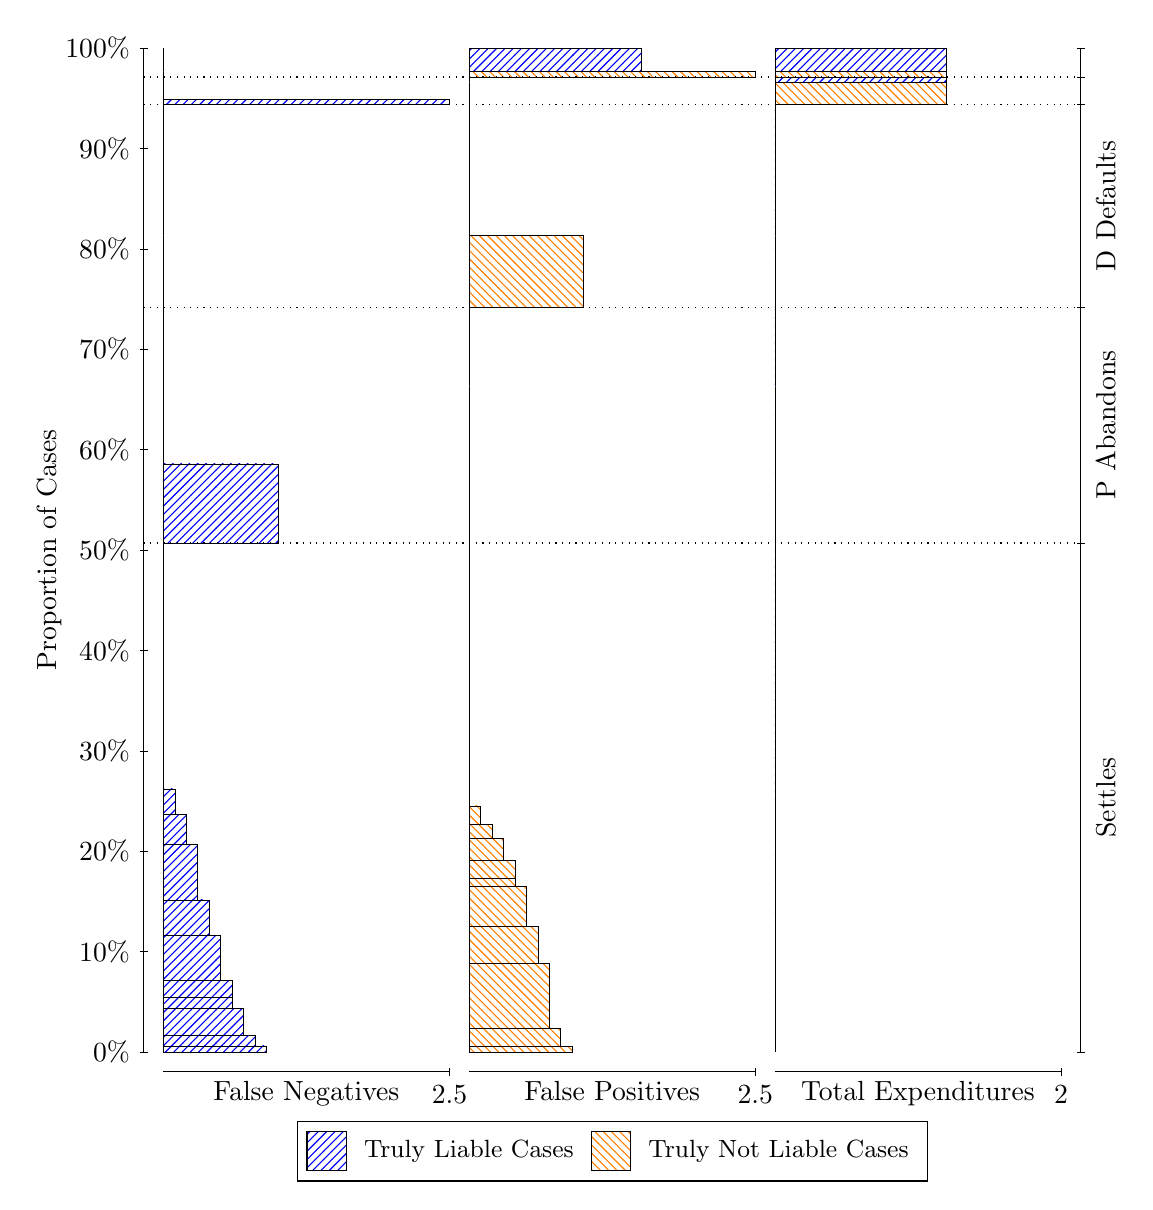
\begin{tikzpicture}
\draw[black, very thin] (1.5,1.75) -- (1.5,14.5);
\node[rotate=90, text=black, anchor=center] at (0.3, 8.125) {Proportion of Cases};
\draw[black, very thin] (1.45,1.75) -- (1.55,1.75);
\node[text=black, anchor=east] at (1.45, 1.75) {0\%};
\draw[black, very thin] (1.45,3.025) -- (1.55,3.025);
\node[text=black, anchor=east] at (1.45, 3.025) {10\%};
\draw[black, very thin] (1.45,4.3) -- (1.55,4.3);
\node[text=black, anchor=east] at (1.45, 4.3) {20\%};
\draw[black, very thin] (1.45,5.575) -- (1.55,5.575);
\node[text=black, anchor=east] at (1.45, 5.575) {30\%};
\draw[black, very thin] (1.45,6.85) -- (1.55,6.85);
\node[text=black, anchor=east] at (1.45, 6.85) {40\%};
\draw[black, very thin] (1.45,8.125) -- (1.55,8.125);
\node[text=black, anchor=east] at (1.45, 8.125) {50\%};
\draw[black, very thin] (1.45,9.4) -- (1.55,9.4);
\node[text=black, anchor=east] at (1.45, 9.4) {60\%};
\draw[black, very thin] (1.45,10.675) -- (1.55,10.675);
\node[text=black, anchor=east] at (1.45, 10.675) {70\%};
\draw[black, very thin] (1.45,11.95) -- (1.55,11.95);
\node[text=black, anchor=east] at (1.45, 11.95) {80\%};
\draw[black, very thin] (1.45,13.225) -- (1.55,13.225);
\node[text=black, anchor=east] at (1.45, 13.225) {90\%};
\draw[black, very thin] (1.45,14.5) -- (1.55,14.5);
\node[text=black, anchor=east] at (1.45, 14.5) {100\%};

\draw[black, very thin] (13.4,1.75) -- (13.4,14.5);
\draw[black, very thin] (13.35,1.75) -- (13.45,1.75);
\node[anchor=west] at (13.35, 1.75) {};
\draw[black, very thin] (13.35,8.2138) -- (13.45,8.2138);
\node[anchor=west] at (13.35, 8.2138) {};
\draw[black, very thin] (13.35,11.209) -- (13.45,11.209);
\node[anchor=west] at (13.35, 11.209) {};
\draw[black, very thin] (13.35,13.782) -- (13.45,13.782);
\node[anchor=west] at (13.35, 13.782) {};
\draw[black, very thin] (13.35,14.132) -- (13.45,14.132);
\node[anchor=west] at (13.35, 14.132) {};
\draw[black, very thin] (13.35,14.5) -- (13.45,14.5);
\node[anchor=west] at (13.35, 14.5) {};

\draw[black, very thin, pattern color=blue, pattern=north east lines] (1.75,1.75) rectangle (3.058,1.8272);
\draw[black, very thin, pattern color=blue, pattern=north east lines] (1.75,1.8272) rectangle (2.9127,1.9583);
\draw[black, very thin, pattern color=blue, pattern=north east lines] (1.75,1.9583) rectangle (2.7673,2.3033);
\draw[black, very thin, pattern color=blue, pattern=north east lines] (1.75,2.3033) rectangle (2.622,2.4417);
\draw[black, very thin, pattern color=blue, pattern=north east lines] (1.75,2.4417) rectangle (2.622,2.6595);
\draw[black, very thin, pattern color=blue, pattern=north east lines] (1.75,2.6595) rectangle (2.4767,3.2304);
\draw[black, very thin, pattern color=blue, pattern=north east lines] (1.75,3.2304) rectangle (2.3313,3.6819);
\draw[black, very thin, pattern color=blue, pattern=north east lines] (1.75,3.6819) rectangle (2.186,4.3825);
\draw[black, very thin, pattern color=blue, pattern=north east lines] (1.75,4.3825) rectangle (2.0407,4.7656);
\draw[black, very thin, pattern color=blue, pattern=north east lines] (1.75,4.7656) rectangle (1.8953,5.0899);
\draw[black, very thin, pattern color=orange, pattern=north west lines] (1.75,5.0899) rectangle (1.75,8.2138);
\draw[black, very thin, pattern color=blue, pattern=north east lines] (1.75,8.2138) rectangle (3.2033,9.2198);
\draw[black, very thin, pattern color=orange, pattern=north west lines] (1.75,9.2198) rectangle (1.75,11.209);
\draw[black, very thin, pattern color=orange, pattern=north west lines] (1.75,11.209) rectangle (1.75,12.121);
\draw[black, very thin, pattern color=blue, pattern=north east lines] (1.75,12.121) rectangle (1.75,13.782);
\draw[black, very thin, pattern color=blue, pattern=north east lines] (1.75,13.782) rectangle (5.3833,13.849);
\draw[black, very thin, pattern color=orange, pattern=north west lines] (1.75,13.849) rectangle (1.75,14.132);
\draw[black, very thin, pattern color=orange, pattern=north west lines] (1.75,14.132) rectangle (1.75,14.199);
\draw[black, very thin, pattern color=blue, pattern=north east lines] (1.75,14.199) rectangle (1.75,14.5);
\draw[black, very thin, pattern color=orange, pattern=north west lines] (5.6333,1.75) rectangle (6.9413,1.8249);
\draw[black, very thin, pattern color=orange, pattern=north west lines] (5.6333,1.8249) rectangle (6.796,2.0537);
\draw[black, very thin, pattern color=orange, pattern=north west lines] (5.6333,2.0537) rectangle (6.6507,2.8731);
\draw[black, very thin, pattern color=orange, pattern=north west lines] (5.6333,2.8731) rectangle (6.5053,3.3442);
\draw[black, very thin, pattern color=orange, pattern=north west lines] (5.6333,3.3442) rectangle (6.36,3.8486);
\draw[black, very thin, pattern color=orange, pattern=north west lines] (5.6333,3.8486) rectangle (6.2147,3.9578);
\draw[black, very thin, pattern color=orange, pattern=north west lines] (5.6333,3.9578) rectangle (6.2147,4.1829);
\draw[black, very thin, pattern color=orange, pattern=north west lines] (5.6333,4.1829) rectangle (6.0693,4.46);
\draw[black, very thin, pattern color=orange, pattern=north west lines] (5.6333,4.46) rectangle (5.924,4.644);
\draw[black, very thin, pattern color=orange, pattern=north west lines] (5.6333,4.644) rectangle (5.7787,4.8739);
\draw[black, very thin, pattern color=blue, pattern=north east lines] (5.6333,4.8739) rectangle (5.6333,8.2138);
\draw[black, very thin, pattern color=orange, pattern=north west lines] (5.6333,8.2138) rectangle (5.6333,10.203);
\draw[black, very thin, pattern color=blue, pattern=north east lines] (5.6333,10.203) rectangle (5.6333,11.209);
\draw[black, very thin, pattern color=orange, pattern=north west lines] (5.6333,11.209) rectangle (7.0867,12.121);
\draw[black, very thin, pattern color=blue, pattern=north east lines] (5.6333,12.121) rectangle (5.6333,13.782);
\draw[black, very thin, pattern color=orange, pattern=north west lines] (5.6333,13.782) rectangle (5.6333,14.065);
\draw[black, very thin, pattern color=blue, pattern=north east lines] (5.6333,14.065) rectangle (5.6333,14.132);
\draw[black, very thin, pattern color=orange, pattern=north west lines] (5.6333,14.132) rectangle (9.2667,14.199);
\draw[black, very thin, pattern color=blue, pattern=north east lines] (5.6333,14.199) rectangle (7.8133,14.5);
\draw[black, very thin, pattern color=orange, pattern=north west lines] (9.5167,1.75) rectangle (9.5167,4.8739);
\draw[black, very thin, pattern color=blue, pattern=north east lines] (9.5167,4.8739) rectangle (9.5167,8.2138);
\draw[black, very thin, pattern color=orange, pattern=north west lines] (9.5167,8.2138) rectangle (9.5167,10.203);
\draw[black, very thin, pattern color=blue, pattern=north east lines] (9.5167,10.203) rectangle (9.5167,11.209);
\draw[black, very thin, pattern color=orange, pattern=north west lines] (9.5167,11.209) rectangle (9.5167,12.121);
\draw[black, very thin, pattern color=blue, pattern=north east lines] (9.5167,12.121) rectangle (9.5167,13.782);
\draw[black, very thin, pattern color=orange, pattern=north west lines] (9.5167,13.782) rectangle (11.697,14.065);
\draw[black, very thin, pattern color=blue, pattern=north east lines] (9.5167,14.065) rectangle (11.697,14.132);
\draw[black, very thin, pattern color=orange, pattern=north west lines] (9.5167,14.132) rectangle (11.697,14.199);
\draw[black, very thin, pattern color=blue, pattern=north east lines] (9.5167,14.199) rectangle (11.697,14.5);
\draw[black, dotted] (1.5,8.2138) -- (13.4,8.2138);
\draw[black, dotted] (1.5,11.209) -- (13.4,11.209);
\draw[black, dotted] (1.5,13.782) -- (13.4,13.782);
\draw[black, dotted] (1.5,14.132) -- (13.4,14.132);
\draw[black, very thin] (1.75,1.5) -- (5.3833,1.5);
\node[text=black, anchor=north] at (3.5667, 1.5) {False Negatives};
\draw[black, very thin] (5.3833,1.45) -- (5.3833,1.55);
\node[text=black, anchor=north] at (5.3833, 1.45) {2.5};

\draw[black, very thin] (5.6333,1.5) -- (9.2667,1.5);
\node[text=black, anchor=north] at (7.45, 1.5) {False Positives};
\draw[black, very thin] (9.2667,1.45) -- (9.2667,1.55);
\node[text=black, anchor=north] at (9.2667, 1.45) {2.5};

\draw[black, very thin] (9.5167,1.5) -- (13.15,1.5);
\node[text=black, anchor=north] at (11.333, 1.5) {Total Expenditures};
\draw[black, very thin] (13.15,1.45) -- (13.15,1.55);
\node[text=black, anchor=north] at (13.15, 1.45) {2};

\node[text=black, centered, rotate=90] at (13.72, 4.9819) {Settles};
\node[text=black, centered, rotate=90] at (13.72, 9.7116) {P Abandons};
\node[text=black, centered, rotate=90] at (13.72, 12.496) {D Defaults};



\draw (7.449999999999999,1.5) node[draw=none] (baseCoordinate) {};
\begin{scope}[align=center]
        \matrix[scale=0.5, draw=black, below=0.5cm of baseCoordinate, nodes={draw}, column sep=0.1cm]{
            \node[rectangle, draw, minimum width=0.5cm, minimum height=0.5cm, pattern color=blue, pattern=north east lines] {}; &
            \node[draw=none, font=\small, text=black] (B) {Truly Liable Cases}; &
            \node[rectangle, draw, minimum width=0.5cm, minimum height=0.5cm, pattern color=orange, pattern=north west lines] {}; &
            \node[draw=none, font=\small, text=black] (B) {Truly Not Liable Cases}; \\
            };
\end{scope}

\end{tikzpicture}
\end{document}